\documentclass[tikz,border=10pt]{standalone}
\usepackage{pgfplots}
\pgfplotsset{compat=1.18}
\usepackage{amsmath,amssymb,bm}
\usetikzlibrary{arrows.meta,positioning,shapes.geometric}
\definecolor{darkbg}{HTML}{ffffff}
\definecolor{lightfg}{HTML}{333333}
\definecolor{accent}{HTML}{2d7d46}
\definecolor{accent2}{HTML}{2d6d7d}
\definecolor{mutedcol}{HTML}{888888}
\definecolor{bordercol}{HTML}{cccccc}
\definecolor{redcol}{HTML}{cc3333}
\definecolor{bluecol}{HTML}{3355bb}
\color{lightfg}

\begin{document}
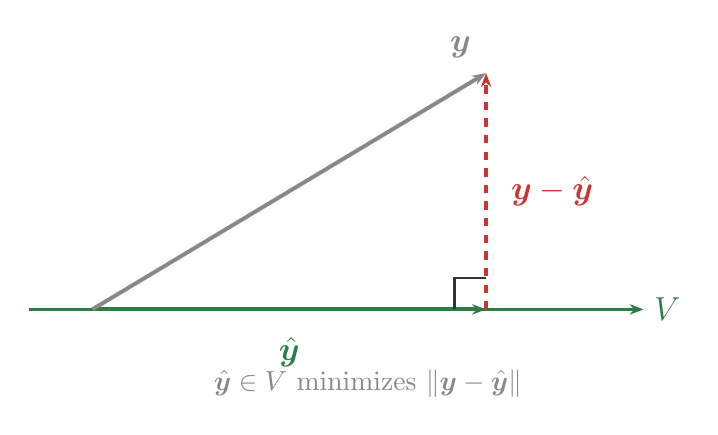
\begin{tikzpicture}[
    >=Stealth,
    thick,
  ]

  \coordinate (O) at (0,0);
  \coordinate (yhat) at (5,0);
  \coordinate (y) at (5,3);

  % Subspace V line
  \draw[accent, -{Stealth[length=5pt]}, line width=1.2pt]
    (-0.8,0) -- (7,0)
    node[right, font=\large\bfseries] {$V$};

  % Projection vector y-hat
  \draw[accent, -{Stealth[length=5pt]}, line width=1.4pt]
    (O) -- (yhat)
    node[midway, below=6pt, accent, font=\large] {$\hat{\bm{y}}$};

  % Original vector y
  \draw[mutedcol, -{Stealth[length=5pt]}, line width=1.4pt]
    (O) -- (y)
    node[above left=2pt, mutedcol, font=\large] {$\bm{y}$};

  % Residual y - y-hat
  \draw[redcol, dashed, line width=1.4pt, -{Stealth[length=5pt]}]
    (yhat) -- (y)
    node[midway, right=5pt, redcol, font=\large] {$\bm{y} - \hat{\bm{y}}$};

  % Right angle mark
  \draw[lightfg, line width=0.8pt]
    (4.6,0) -- (4.6,0.4) -- (5,0.4);

  % Caption
  \node[below=18pt, mutedcol, font=\normalsize] at (3.5,0)
    {$\hat{\bm{y}} \in V$ minimizes $\|\bm{y} - \hat{\bm{y}}\|$};

\end{tikzpicture}
\end{document}
